\chapter{Requirements and Specifications}
\section{Block Diagram}

\begin{figure}[H]
\centering
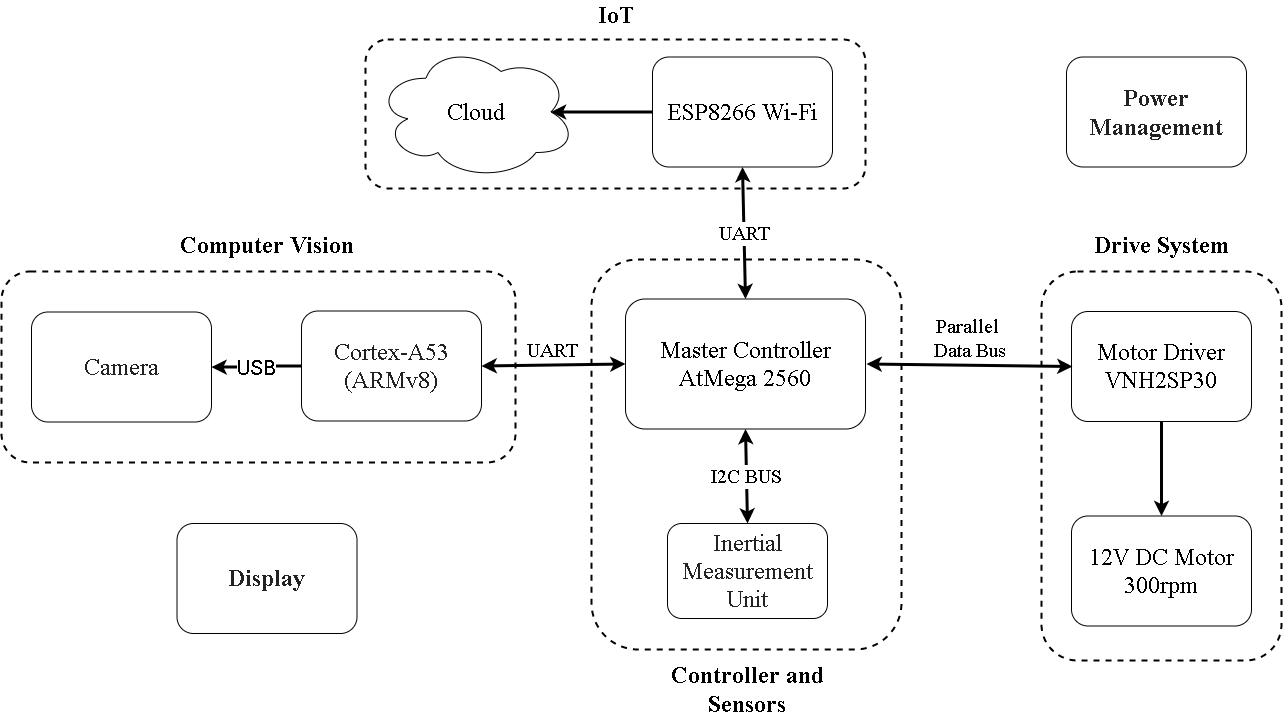
\includegraphics[width = \textwidth]{project/images/blockdiagram.png}
\caption{Block Diagram} \label{blockdiagram}
\end{figure}
\newpage

\section{Software}
\subsection{AutoDesk Fusion}
\paragraph{}Fusion 360™ is a cloud-based 3D CAD/CAM tool for product development that combines industrial and mechanical design, collaboration, and machining in a single package. Fusion 360 enables fast and easy exploration of design ideas with an integrated concept-to-production platform. % Refer Appendix \ref{fusion360} for more information.

Version used - \textit{2020 January - Student Version}

\begin{figure}[H]
\centering
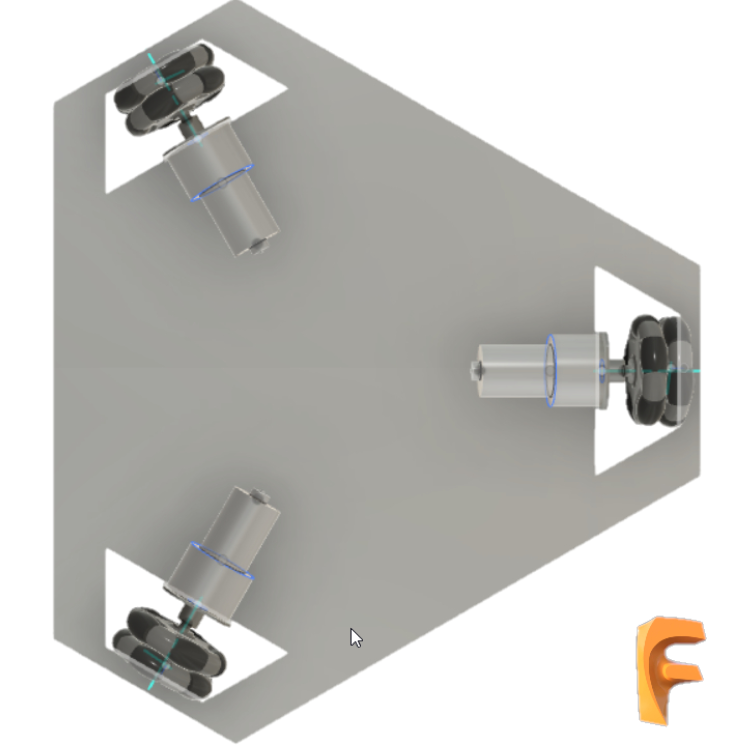
\includegraphics[width = 6cm]{project/images/chassis_3d_model.png}
\caption{3D Model of chassis created in Autodesk Fusion 360™} \label{chassis}
\end{figure}

\subsection{AutoDesk Eagle}
\paragraph{}EAGLE is an electronic design automation (EDA) software. Enabling printed circuit board (PCB) designers to seamlessly connect schematic diagrams, component placement, PCB routing and comprehensive library content. % Refer Appendix \ref{eagle} for more information.

Version used - \textit{2020 January - Student Version}

\begin{figure}[H]
\centering
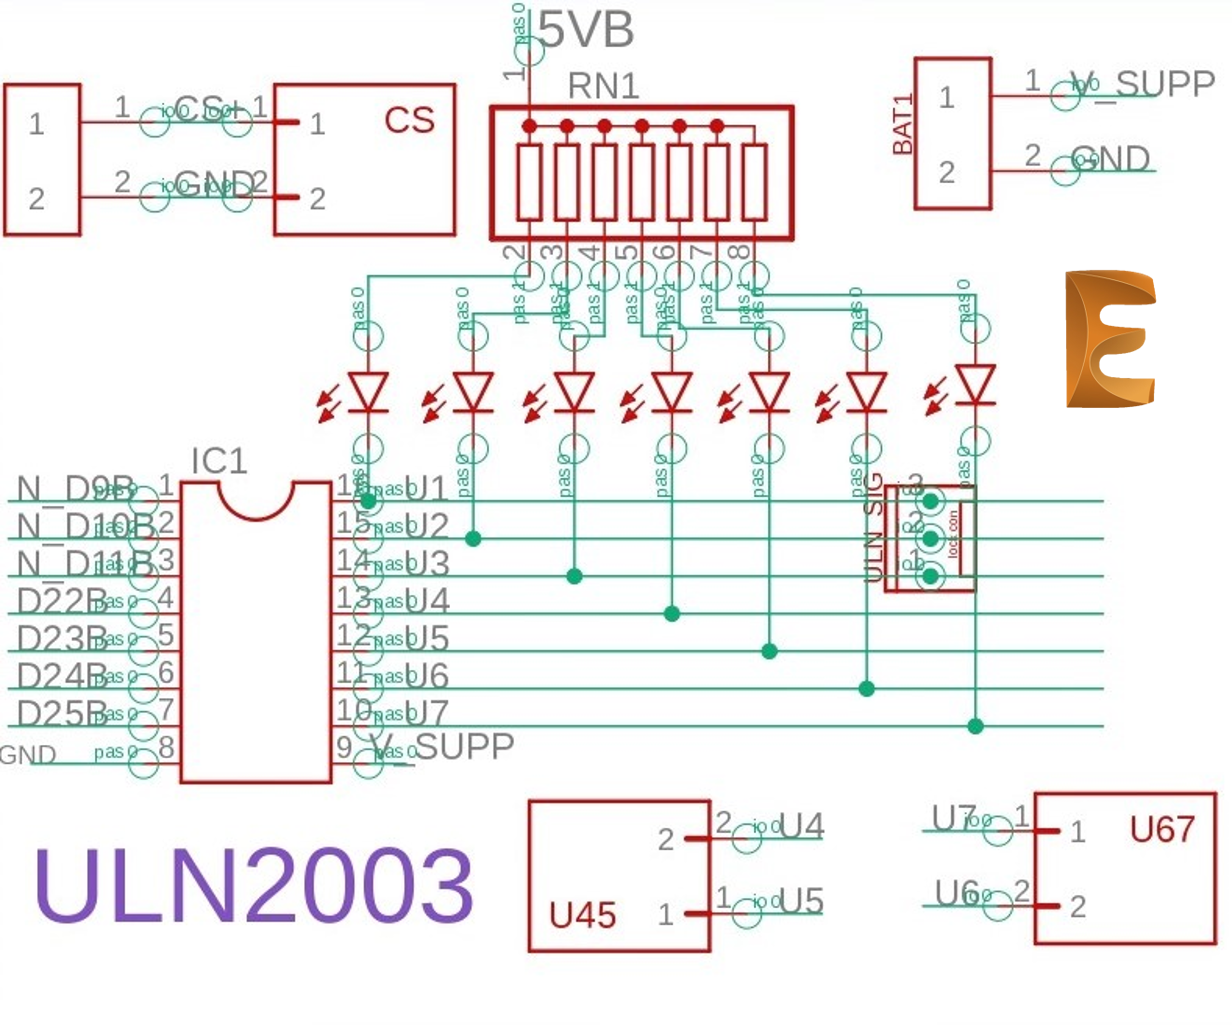
\includegraphics[width = 6cm]{project/images/uln2003.png}
\caption{Electronics schematic designed in Autodesk Eagle}\label{uln2003}
\end{figure}

\subsection{Arduino IDE}
\paragraph{}The Arduino Integrated Development Environment (IDE) is a cross-platform application (for Windows, macOS, Linux) that is written in functions from C and C++. It is used to write and upload programs to Arduino compatible boards, but also, with the help of 3rd party cores, other vendor development boards. % Refer Appendix \ref{arduinoide} for more information.

Version used - \textit{Arduino 1.8.9}

\begin{figure}[H]
\centering

\includegraphics[width = 6cm]{project/images/arduino_ide.png}
\caption{Arduino IDE}
\end{figure}

\subsection{Python IDLE}
\paragraph{}

IDLE is Python’s Integrated Development and Learning Environment.\\
IDLE has the following features:

\begin{itemize}
    \item coded in 100\% pure Python, using the tkinter GUI toolkit
    
    \item cross-platform: works mostly the same on Windows, Unix, and macOS
    
    \item multi-window text editor with multiple undo, Python colorizing, smart indent, call tips, auto completion, and other features
    
    \item search within any window, replace within editor windows, and search through multiple files (grep)
    
    \item debugger with persistent breakpoints, stepping, and viewing of global and local namespaces

\end{itemize}
% Refer Appendix \ref{pythonidle} for more information. 
Version used - \textit{Python 3.7.6}

\begin{figure}[H]
\centering
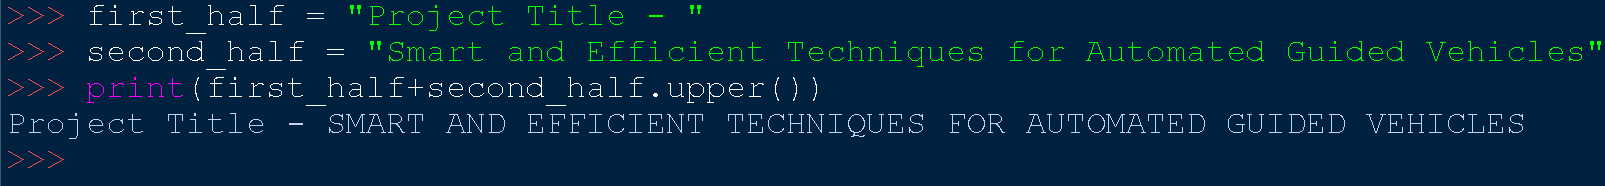
\includegraphics[width = \textwidth]{project/images/python_idle.png}
\caption{Python IDLE}
\end{figure}

\subsection{Raspbian}
\paragraph{}Raspbian is the Foundation’s official supported operating system. Raspbian comes pre-installed with plenty of software for education, programming and general use. It has \textbf{Python}, Scratch, Sonic Pi, Java and more. % Refer Appendix \ref{raspbian} for more information.

Image used - \textit{Raspbian Buster with Desktop and recommended software}

Version used - \textit{September 2019}

\begin{figure}[H]
\centering
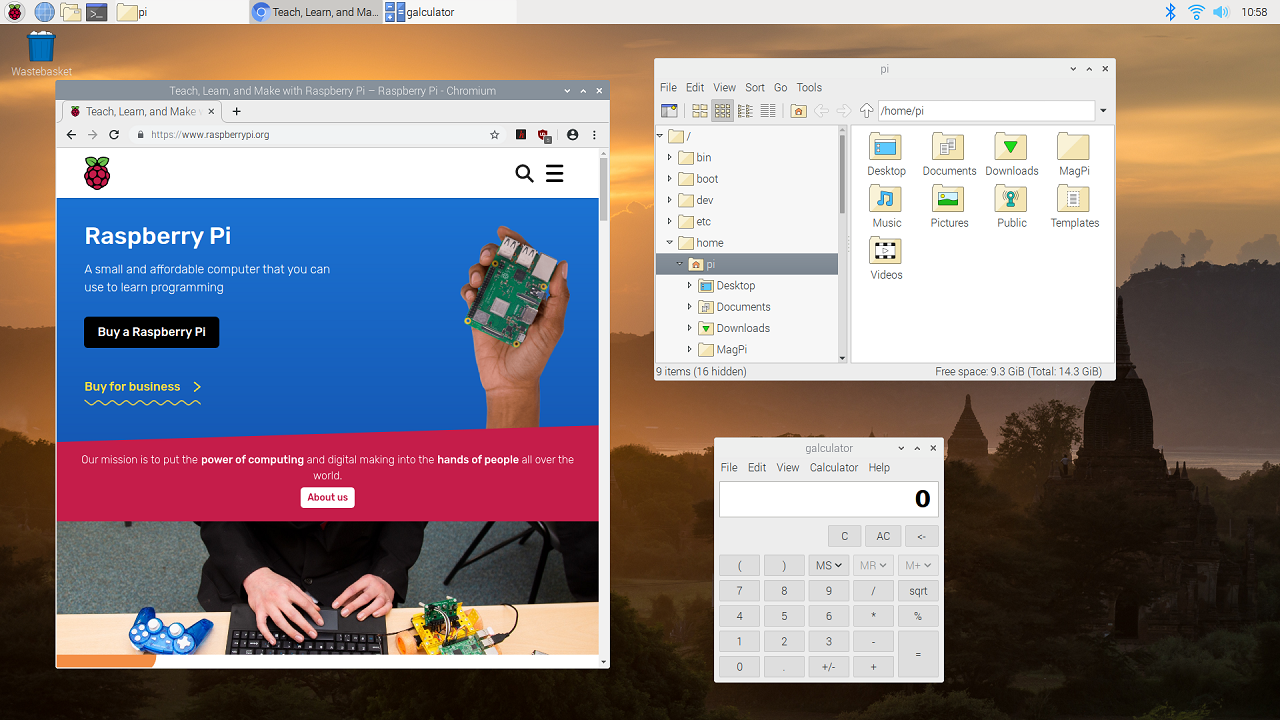
\includegraphics[width = \textwidth]{project/images/raspbian.png}
\caption{Rasbian Buster}
\end{figure}

First step after booting 

\begin{verbatim}
  $ sudo apt update
  $ sudo apt upgrade
\end{verbatim}

Creating Virtual Environment

\begin{verbatim}
  $ sudo pip3 install virtualenv
  $ python3 -m venv virtual-env
  $ source virtual-env/bin/activate
\end{verbatim}

% For Object Detection using TensorFlow Lite in Raspberry Pi, refer Appendix \ref{edjeelectronics}.
\newpage
\subsection{Anaconda}
\begin{itemize}
    \item Free \& Open Source distribution of Python
    \item Packages for Scientific Computing
    \item ML \& Data Science Libraries out of the box
\end{itemize}

Version used - \textit{2019.10 for 64-bit Windows with Python 3.7}

\begin{verbatim}
  conda install -c anaconda tensorflow-gpu
\end{verbatim}

% \begin{figure}[H]
% \centering
% 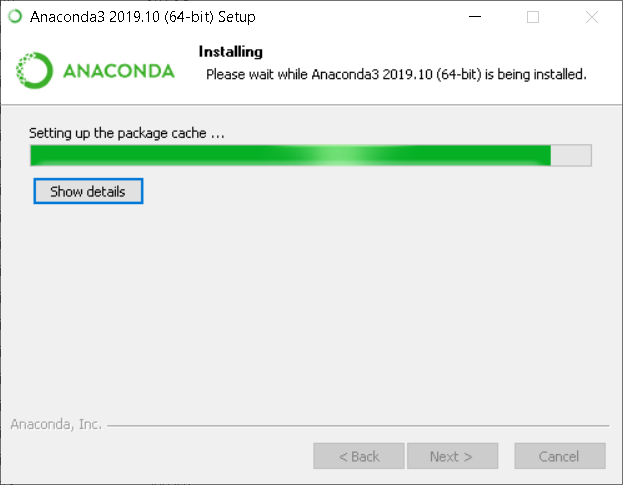
\includegraphics[width = 9cm]{project/images/anaconda.PNG}
% \caption{Anaconda Installation}
% \end{figure}

\subsection{TensorFlow}

\begin{itemize}
    \item An end-to-end open source machine learning platform
    \item Comprehensive, flexible ecosystem of tools, libraries and community resources
    \item Lets researchers push the state-of-the-art in ML
    \item Developers easily build and deploy ML powered applications
\end{itemize}

\textbf{Specs of Laptop that we used for Tensorflow: }
\begin{itemize}
    \item \textbf{GPU} - GTX 1050 Ti
    \item \textbf{CPU} - CORE i7 8th Gen
    \item \textbf{RAM} - 16 GB
\end{itemize}

\begin{figure}[H]
\centering
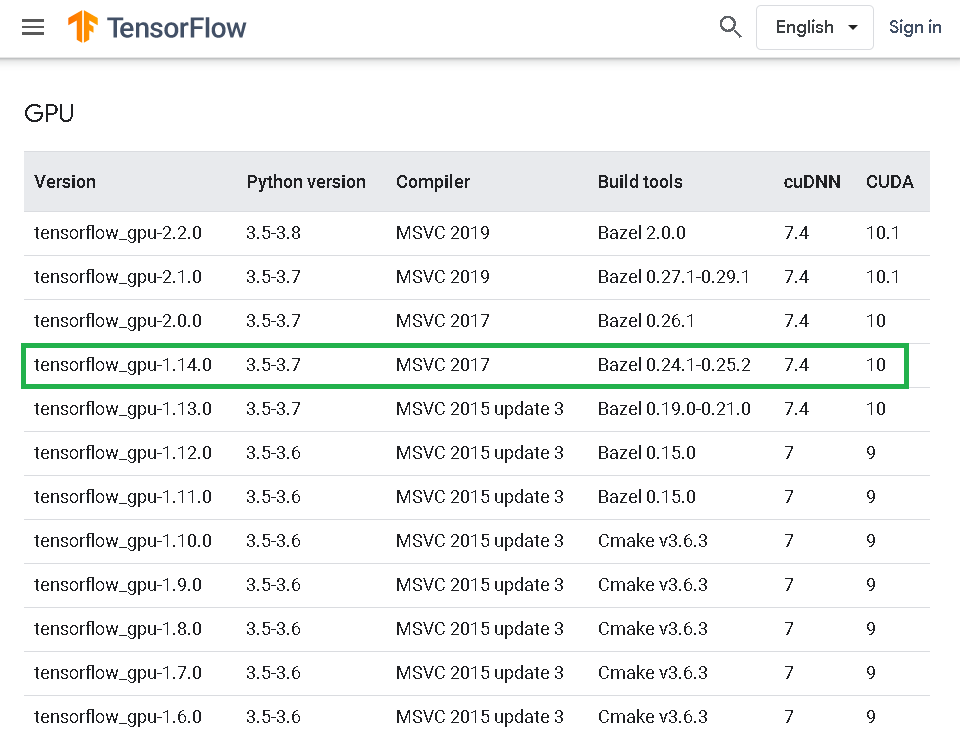
\includegraphics[width = 11cm]{project/images/tensorflow_version.png}
\caption{TensorFlow Configuration}
\end{figure}

\section{Hardware}

\subsection{Micro-controller and Micro-processor}
\begin{itemize}[wide, labelwidth=!, labelindent=0pt]
    \item \textbf{Arduino MEGA}
    \vspace{-0.5cm}
    \paragraph{}The Arduino MEGA 2560 is designed for projects that require more I/O lines, more sketch memory and more RAM. With 54 digital I/O pins, 16 analog inputs and a larger space for your sketch it is the recommended board for 3D printers and robotics projects. This gives your projects plenty of room and opportunities maintaining the simplicity and effectiveness of the Arduino platform.

    \begin{figure}[H]
    \centering
    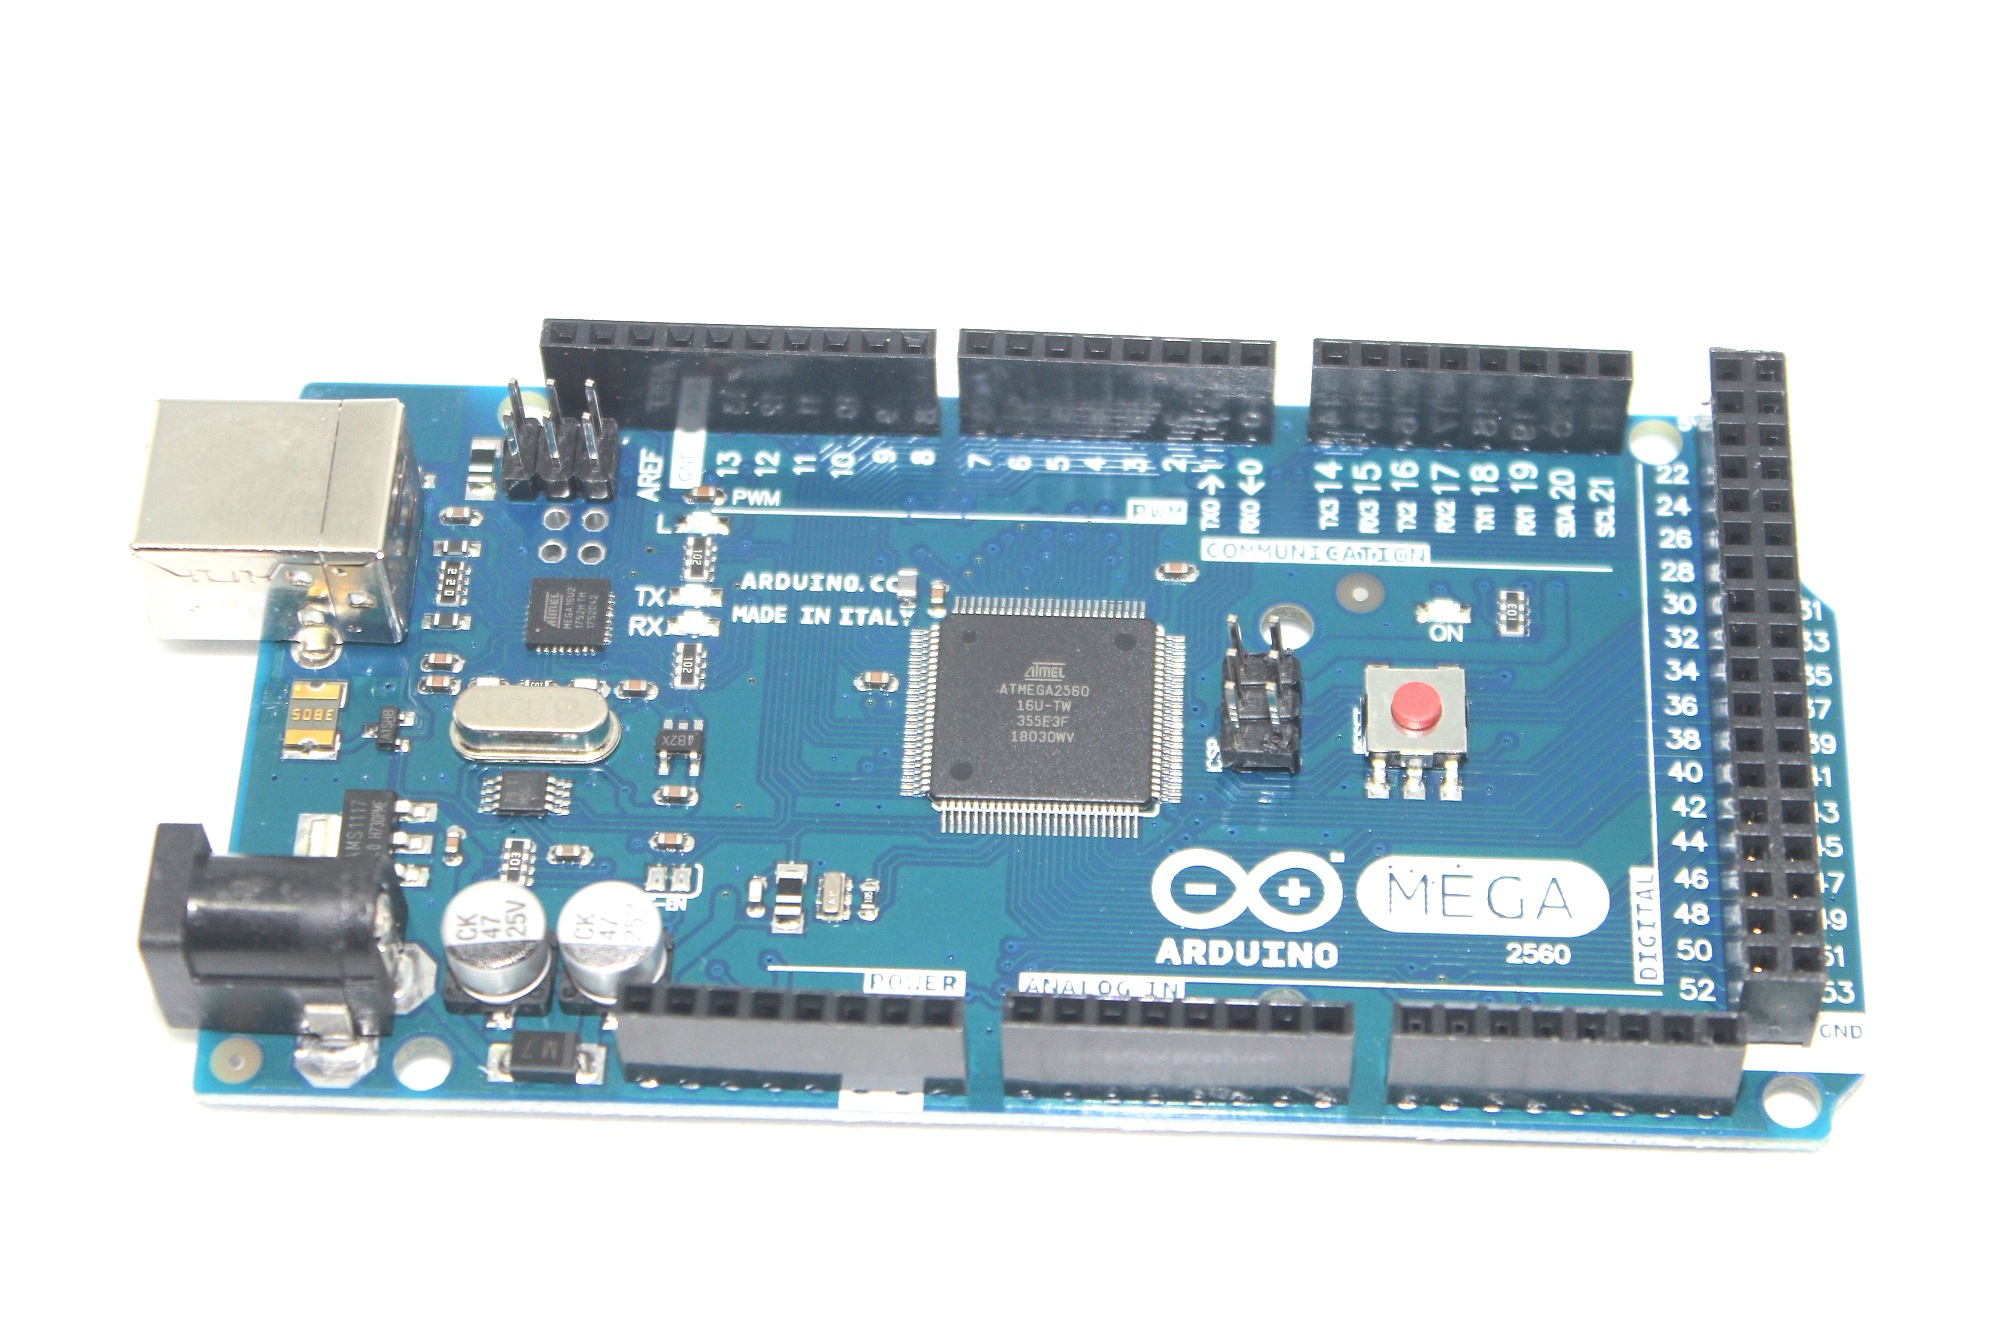
\includegraphics[width = 11cm]{project/images/arduino_mega.jpg}
    \caption{Arduino MEGA 2560}
    \end{figure}
    
    \begin{table}[htbp]
    \caption{Specification of Arduino Mega}
    \begin{center}
    \begin{tabular}{|p{5cm}|p{9cm}|}
    \hline Chip & ATmega2560\\
    \hline Operating Voltage & 5V\\
    \hline Input Voltage & 7-12V\\
    \hline Digital I/O Pins & 54 (of which 14 provide PWM output)\\
    \hline DC Current per I/O Pin & 40 mA\\
    \hline DC Current for 3.3V Pin & 50 mA\\
    \hline Flash Memory & 256 KB of which 8 KB used by bootloader\\
    \hline SRAM & 8KB\\
    \hline EEPROM & 4KB\\
    \hline Clock Speed & 16 MHz\\
    \hline
    \end{tabular}
    \end{center}
    \end{table}
    
    \newpage
    
    \item \textbf{Raspberry Pi 4}
    \vspace{-0.5cm}
    \paragraph{}The Raspberry Pi 4 Model B is the latest version of the low-cost Raspberry Pi computer. The Pi isn't like your typical device; in its cheapest form it doesn't have a case, and is simply a credit-card sized electronic board -- of the type you might find inside a PC or laptop, but much smaller.
    
    The Raspberry Pi 4 can do a surprising amount. Amateur tech enthusiasts use Pi boards as media centers, file servers, retro games consoles, routers, and network-level ad-blockers, for starters. However that is just a taste of what's possible. 
    
    \begin{figure}[H]
    \centering
    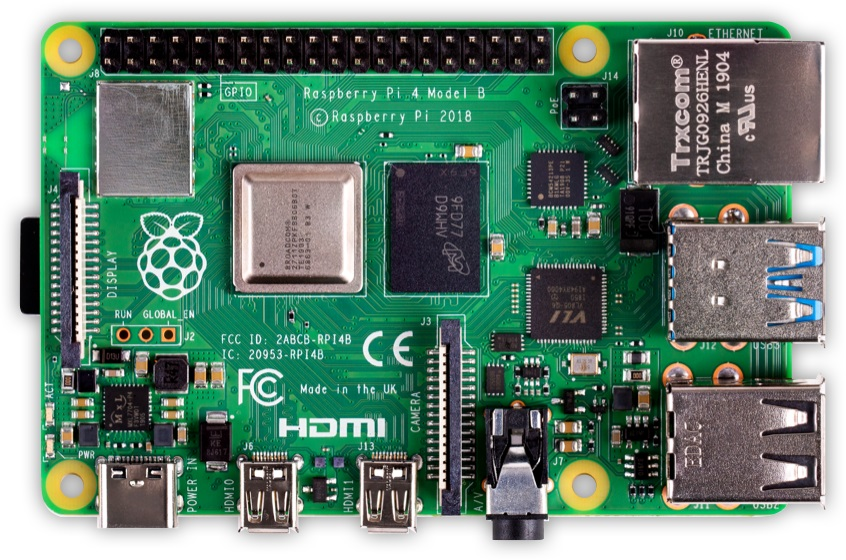
\includegraphics[width = 11cm]{project/images/raspberry_4_B.jpg}
    \caption{Raspberry Pi 4 Model B}
    \end{figure}
    
    \begin{center}{\textbf{Specifications}}\end{center}
    
    \begin{itemize}
        \item Broadcom BCM2711, Quad core Cortex-A72 (ARM v8) 64-bit SoC @ 1.5GHz
        \item 2GB LPDDR4-3200 SDRAM (depending on model)
        \item 2.4 GHz and 5.0 GHz IEEE 802.11ac wireless, Bluetooth 5.0, BLE
        \item Raspberry Pi standard 40 pin GPIO header (fully backwards compatible with previous boards)
        \item H.265 (4kp60 decode), H264 (1080p60 decode, 1080p30 encode)
        \item Micro-SD card slot for loading operating system and data storage
        \item Operating temperature: 0 – 50 degrees C ambient
    \end{itemize}
    
    * A good quality 2.5A power supply can be used if downstream USB peripherals consume less than 500mA in total.
    
    \newpage
    
    \item \textbf{Arduino Nano}
    \vspace{-0.5cm}
    \paragraph{}The Nano is a small, complete, and breadboard-friendly board based on the ATmega328 (Arduino Nano R3). It has more or less the same functionality of the Arduino Uno but in a different package. It lacks only a DC power jack and works with a Mini-B USB cable instead of a standard one.
    
    \begin{figure}[H]
    \centering
    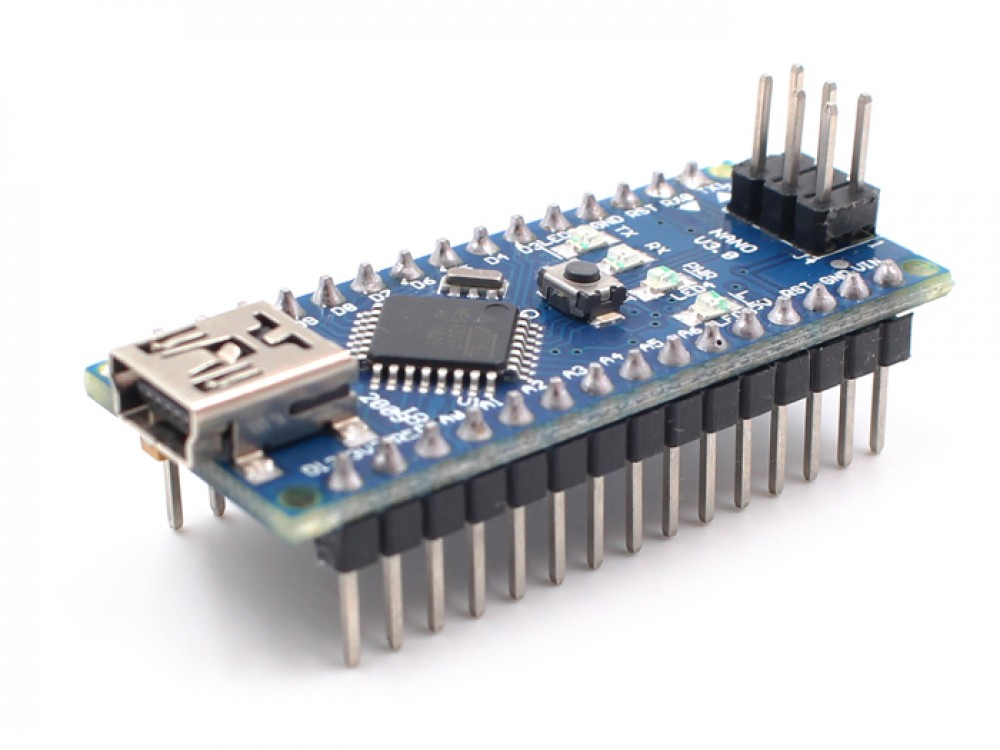
\includegraphics[width = 7cm]{project/images/arduino nano.jpg}
    \caption{Arduino Nano}
    \end{figure}
    
    \item \textbf{Node MCU}
    \vspace{-0.5cm}
    \paragraph{}NodeMCU is an open source firmware for which open source prototyping board designs are available. The name "NodeMCU" combines "node" and "MCU" (micro-controller unit). The term "NodeMCU" strictly speaking refers to the firmware rather than the associated development kits.
    
    \begin{figure}[H]
    \centering
    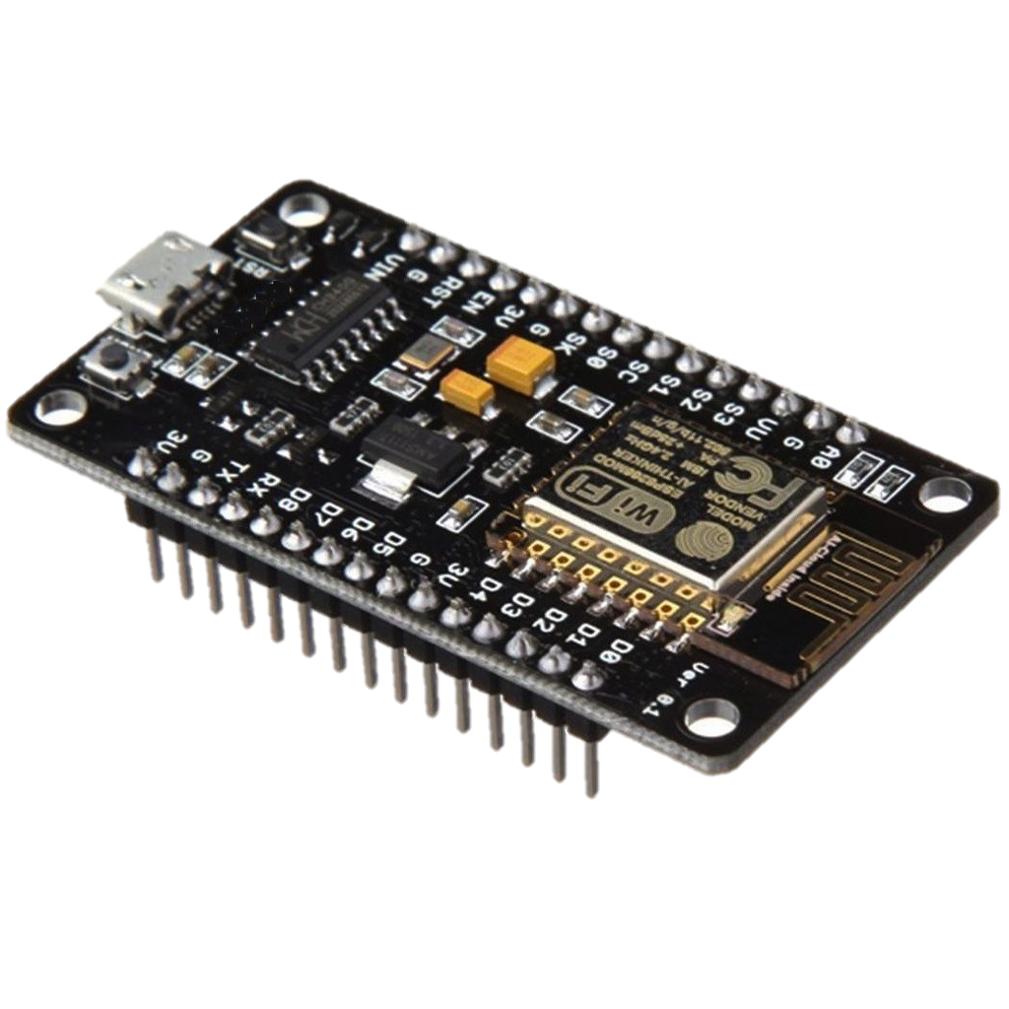
\includegraphics[width = 7cm]{project/images/nodemcu.png}
    \caption{Node MCU}
    \end{figure}
\end{itemize}

\newpage

\subsection{Displays}

\begin{itemize}[wide, labelwidth=!, labelindent=0pt]
    \item \textbf{LCD 1602 Display}
    \vspace{-0.5cm}
    \paragraph{}LCD1602, or 1602 character-type liquid crystal display, is a kind of dot matrix module to show letters, numbers, and characters and so on. It's composed of 5x7 or 5x11 dot matrix positions; each position can display one character.
    \begin{figure}[H]
    \centering
    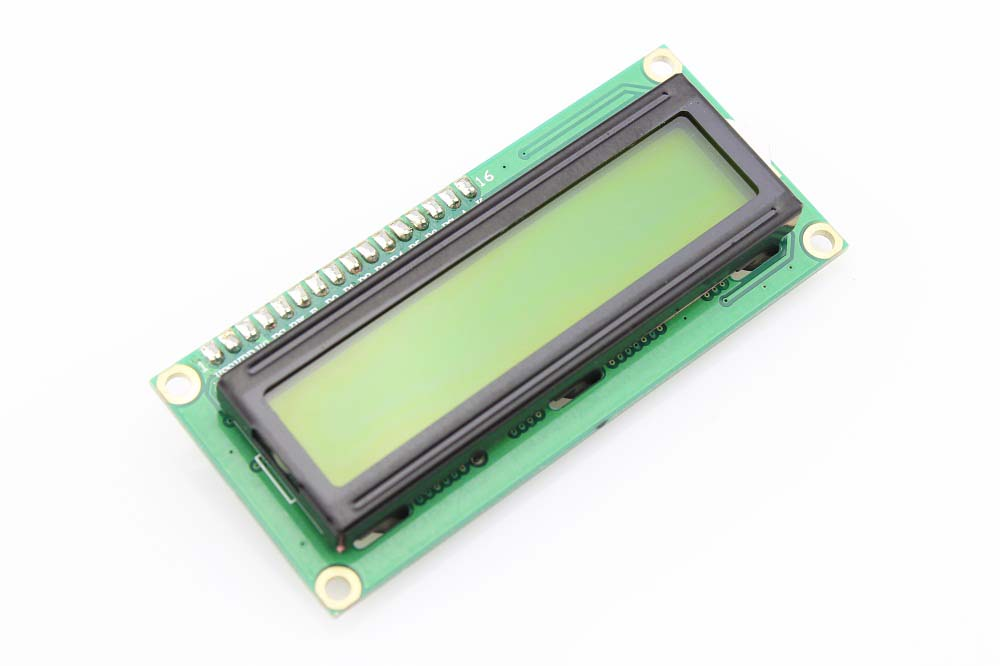
\includegraphics[width = 9cm]{project/images/lcd1602.jpg}
    \caption{LCD 1602 Display}
    \end{figure}
    
    \item \textbf{TM1637 4-digit 7-segment display}
    \vspace{-0.5cm}
    \paragraph{}TM1637 DISPLAY module is used for displaying numbers. The module consists of four 7- segment displays working together. The module working is based on ‘TM1637’ IC present internally and hence the name ‘TM1637 display’.
    \begin{figure}[H]
    \centering
    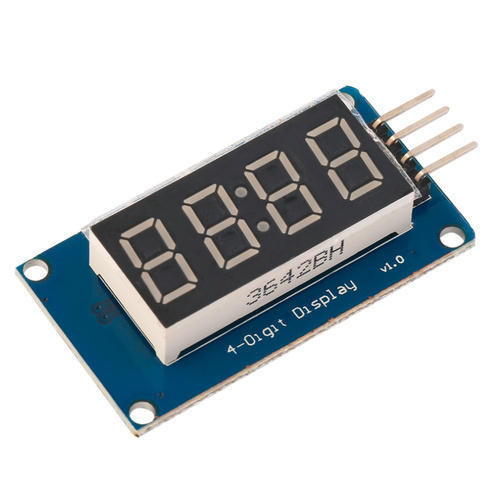
\includegraphics[width = 7cm]{project/images/tm1637.jpg}
    \caption{TM1637 Display}
    \end{figure}

\end{itemize}

\newpage

\subsection{Sensors}

\begin{itemize}[wide, labelwidth=!, labelindent=0pt]
    \item \textbf{L3GD20H Gyroscope}
    \vspace{-0.5cm}
    \paragraph{}The L3GD20H is a low-power three-axis angular rate sensor. It includes a sensing element and an IC interface able to provide the measured angular rate to the external world through digital interface (I2C/SPI). The sensing element is manufactured using a dedicated micromachining process developed by ST to produce inertial sensors and actuators on silicon wafers. The IC interface is manufactured using a CMOS process that allows a high level of integration to design a dedicated circuit which is trimmed to better match the sensing element characteristics. 
    
    \begin{figure}[H]
    \centering
    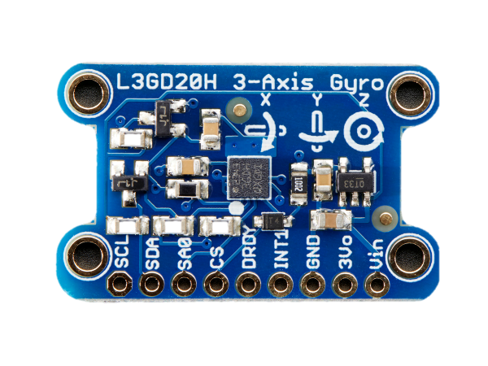
\includegraphics[width = 7cm]{project/images/L3GD20H.jpg.png}
    \caption{L3GD20H Gyroscope}
    \end{figure}
    
    \begin{center}{\textbf{Key Features}}\end{center}
    
    \begin{itemize}
        \item Wide supply voltage, 2.2 V to 3.6 V
        \item Wide extended operating temperature range (from -40 °C to 85 °C)
        \item Low power consumption
        \item Embedded 32 levels of 16 bit data output FIFO
        \item Three selectable full scales up to 2000 dps
        \item 16 bit rate value data output
        \item 8 bit temperature data output
        \item Sleep mode
        \item Fast turn-on and wake-up
    \end{itemize}
    
    \newpage
    
    \item \textbf{Logitech C270}
    \vspace{-0.5cm}
    \paragraph{}The Logitech C270 HD Webcam is a high utility device that helps you to enjoy seamless video calling. This device comes with easy installation process that offers a hassle-free set up. The ergonomic design and sleek body helps in saving space and makes it easy to install the webcam on your PC or laptop. The adjustable design makes it easy to tilt and use it according to your needs. It features 'Logitech Fluid Crystal Technology' and has a 3 MP camera which enhances picture quality while the integrated microphone delivers perfect sound quality.
    
    
    \begin{figure}[H]
    \centering
    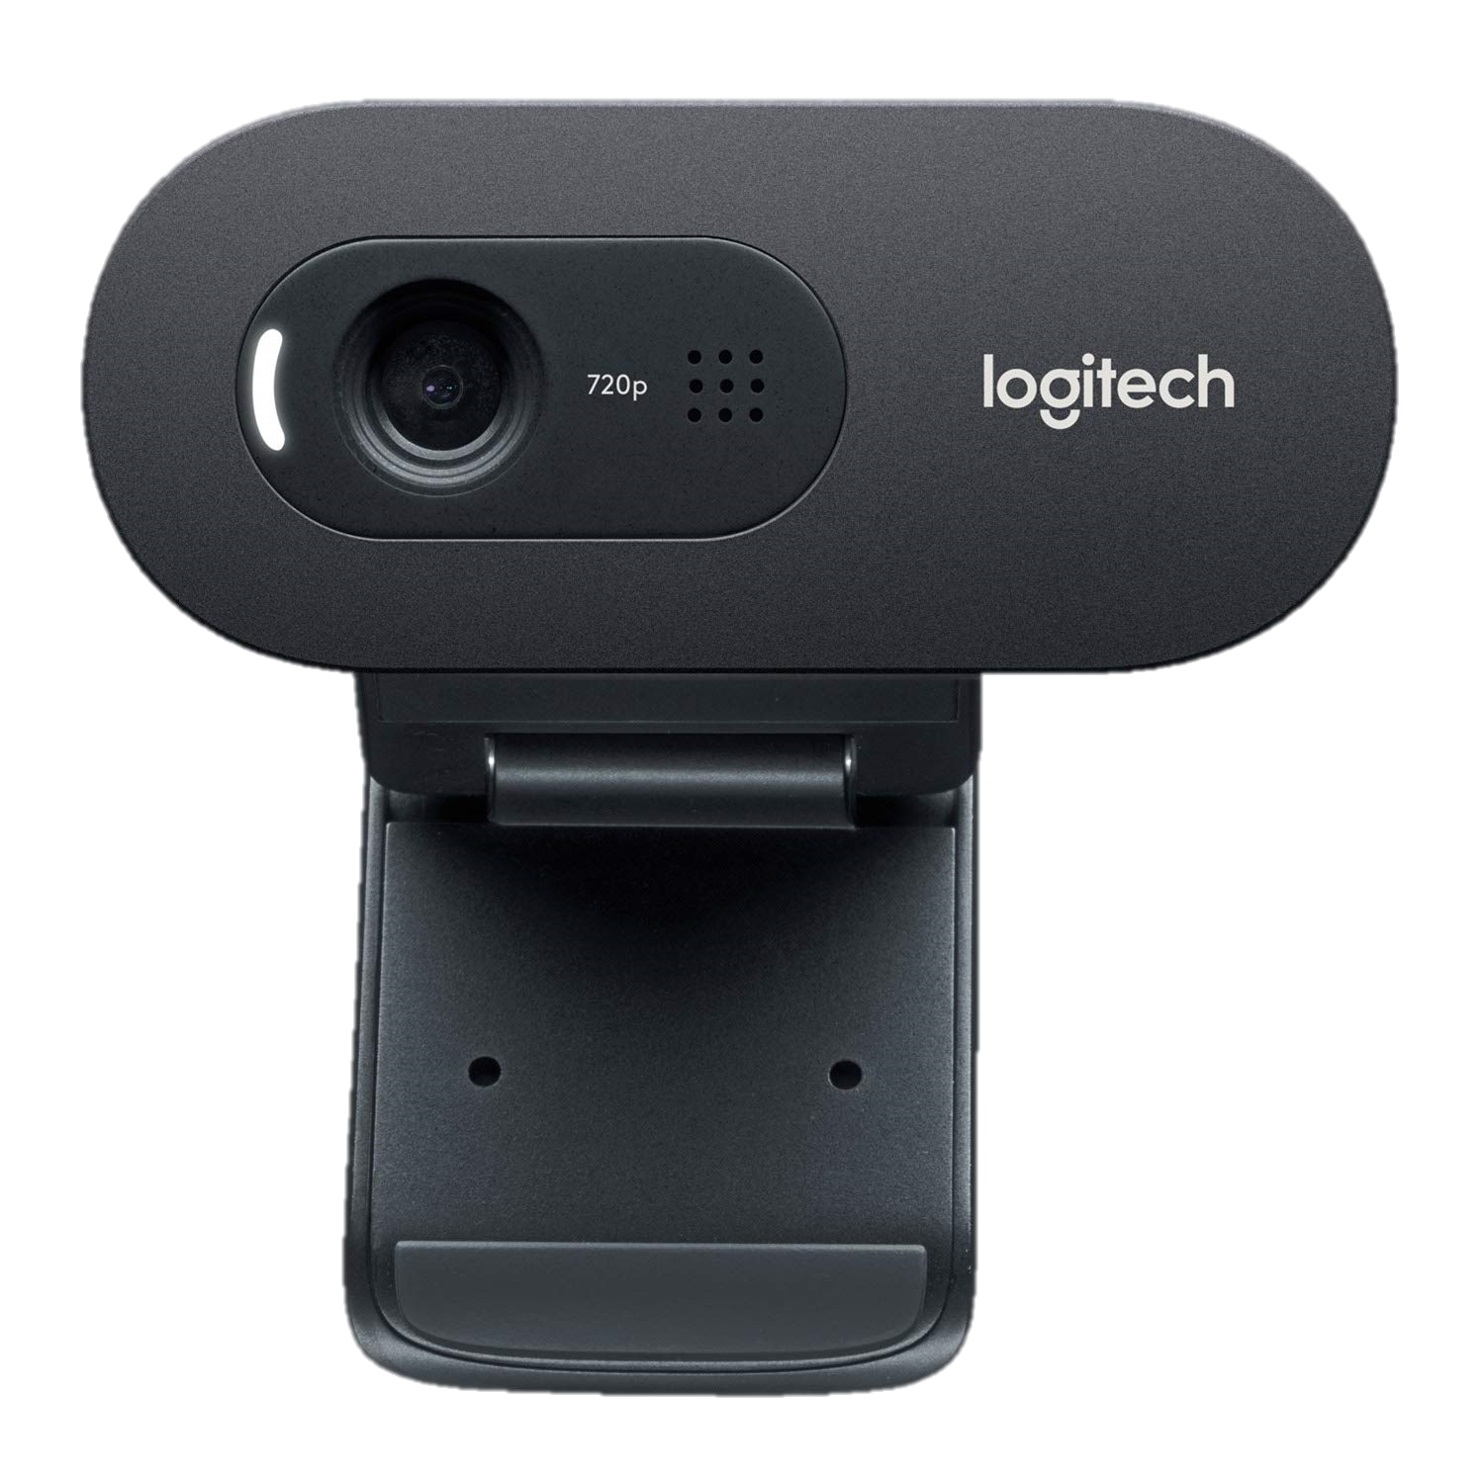
\includegraphics[width = 7cm]{project/images/webcam.jpg}
    \caption{Logitech C270}
    \end{figure}
    
    \begin{center}{\textbf{Technical Specifications}}\end{center}
    
    \begin{itemize}
        \item Max Resolution: 720p/30fps
        \item Focus type: fixed focus
        \item Built-in mic: mono
        \item FoV: 60 degree
        \item Universal clip fits laptops, LCD or monitors
    \end{itemize}

\end{itemize}

\newpage

\subsection{Buck and Boost Converter}

\begin{itemize}[wide, labelwidth=!, labelindent=0pt]
    \item \textbf{Buck LM2596}
    \vspace{-0.5cm}
    \paragraph{}DC-DC Buck Converter Step Down Module LM2596 Power Supply is a step-down(buck) switching regulator, capable of driving a 3-A load with excellent line and load regulation. These devices are available in fixed output voltages of 3.3 V, 5 V, 12 V, and an adjustable output version.
    
    \begin{figure}[H]
    \centering
    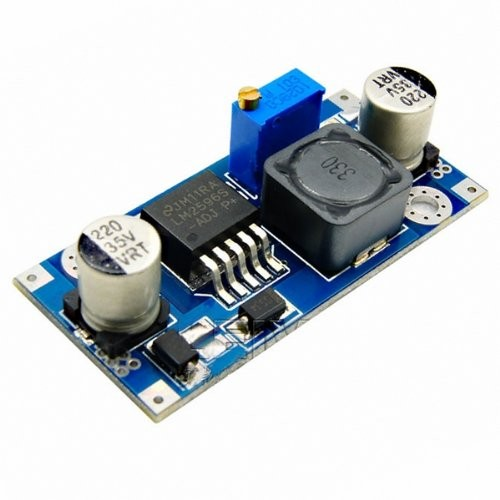
\includegraphics[width = 6cm]{project/images/lm2596.jpg}
    \caption{LM2596}
    \end{figure}
    
    
    \item \textbf{Booster XL6009}
    \vspace{-0.5cm}
    \paragraph{}This CN6009 XL6009 DC – DC Step-up converter module is a non-isolated step-up (boost) voltage converter featuring adjustable output voltage and high efficiency. The module uses the second generation of high-frequency switching technology XL6009E1 core chip performance than the first generation technology LM2577. XL6009 boost module at a lower cost, superior performance. It equips 4A high-efficiency MOSFET switches, so as to provide a conversion efficiency of up to 94\%.
    
    \begin{figure}[H]
    \centering
    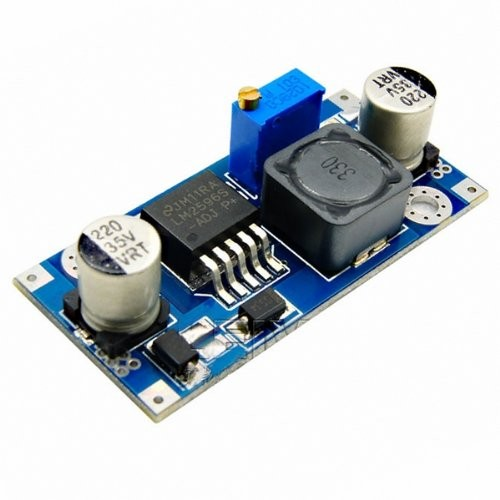
\includegraphics[width = 6cm]{project/images/lm2596.jpg}
    \caption{XL6009}
    \end{figure}

\end{itemize}

\subsection{Motor Drivers}

\begin{itemize}[wide, labelwidth=!, labelindent=0pt]
    \item \textbf{VNH2SP30}
    \vspace{-0.5cm}
    \paragraph{}Monster Moto Shield VNH2SP30 Motor Driver 14A is essentially a ramped up version of our Ardumoto motor driver shield. For this Monster Moto Shield, we’ve replaced the L298 H-bridge with a pair of VNH2SP30 full-bridge motor drivers. We’ve also beefed up the support circuitry so this board is capable of driving a pair of high-current motors! The VIN and motor out are pitched for our 5mm screw terminals (not included), making it easy to connect larger gauge wires.
    
    \begin{figure}[H]
    \centering
    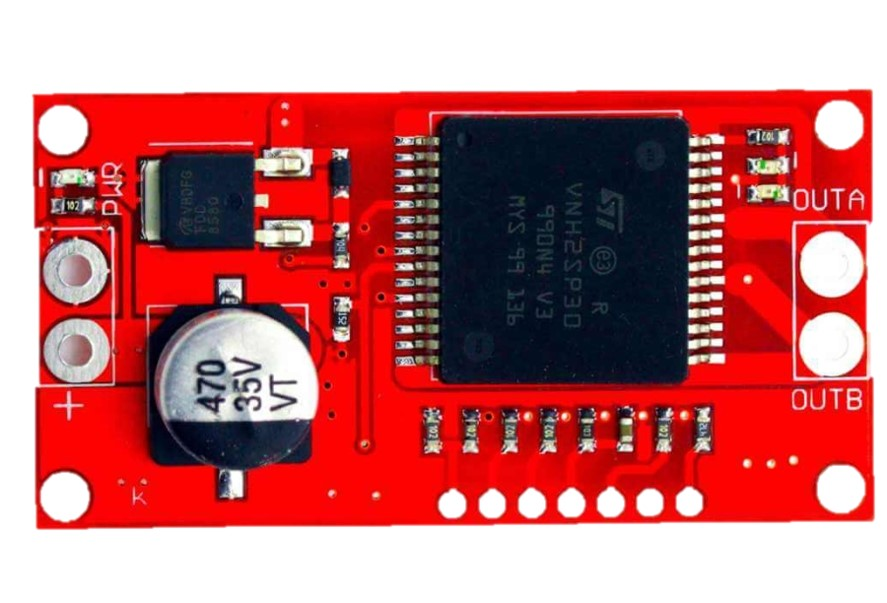
\includegraphics[width = 8cm]{project/images/vnh.jpg}
    \caption{Motor Driver}
    \end{figure}
    
    \begin{center}{\textbf{Technical Specifications}}\end{center}
    
    \begin{itemize}
        \item Voltage Max: 16V
        \item Maximum current rating: 30 A
        \item Practical Continuous Current: 14 A
        \item Current sensing available to Arduino analog pin
        \item MOSFET on-resistance: 19 mΩ (per leg)
        \item Maximum PWM frequency: 20 kHz
        \item Undervoltage and Overvoltage shutdown.
    \end{itemize}

\end{itemize}

\newpage

\subsection{Power Source}

\begin{itemize}[wide, labelwidth=!, labelindent=0pt]
    \item \textbf{LiPo 12V 8000mAh 3S}
    \vspace{-0.5cm}
    \paragraph{}Orange batteries are known for performance, reliability and price. It’s no surprise to us that Orange Lithium polymer packs are the go-to pack for those in the know. Orange batteries deliver the full rated capacity at a price everyone can afford. Orange batteries are equipped with heavy duty discharge leads to minimize resistance and sustain high current loads.
    
    \begin{figure}[H]
    \centering
    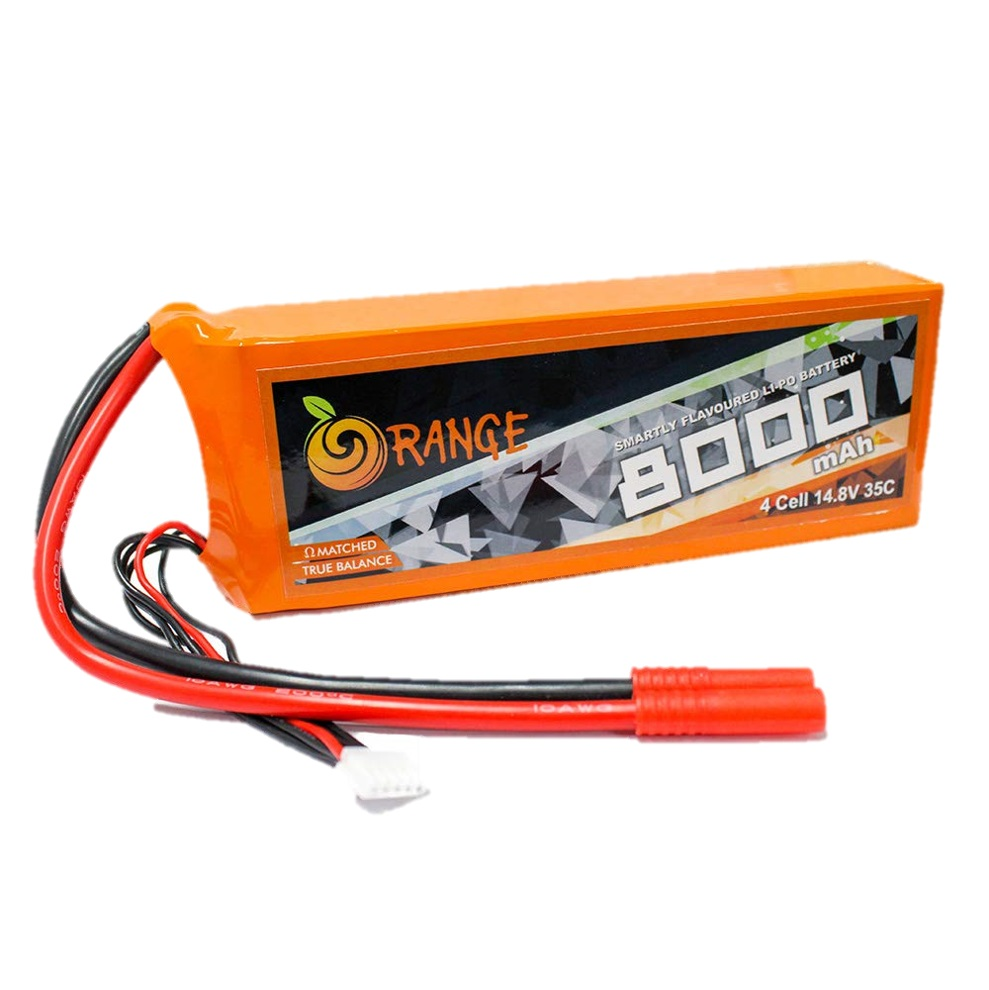
\includegraphics[width = 8cm]{project/images/battery.jpg}
    \caption{LiPo Battery}
    \end{figure}
    
    \begin{center}{\textbf{Specifications}}\end{center}
    
    \begin{itemize}
        \item Model No: ORANGE 8000/3S-30C
        \item Weight : 615.0g
        \item Voltage : 11.1V
        \item Dimensions : 52x43x137 (mm)
        \item Max Continuous Discharge : 30C(240.0A)
        \item Balance Plug : JST-XH
        \item Max Burst Discharge : 60C(480.0A)
        \item Discharge Plug : HXT-4mm
    \end{itemize}

\end{itemize}

\newpage

\subsection{Motors}

\begin{itemize}[wide, labelwidth=!, labelindent=0pt]
    \item \textbf{12V Johnson Geared Motor}
    \vspace{-0.5cm}
    \paragraph{}These are the enhanced quality motors by Orange. The Orange has carefully manufactured this Johnson Geared Motor with the best quality material to give you said torque at said RPM.
    
    This motor is a simple DC motor coupled with Metal Gearbox for delivering more power/torque. Compact size and massive torque make them stand tall in the market. 

    \begin{figure}[H]
    \centering
    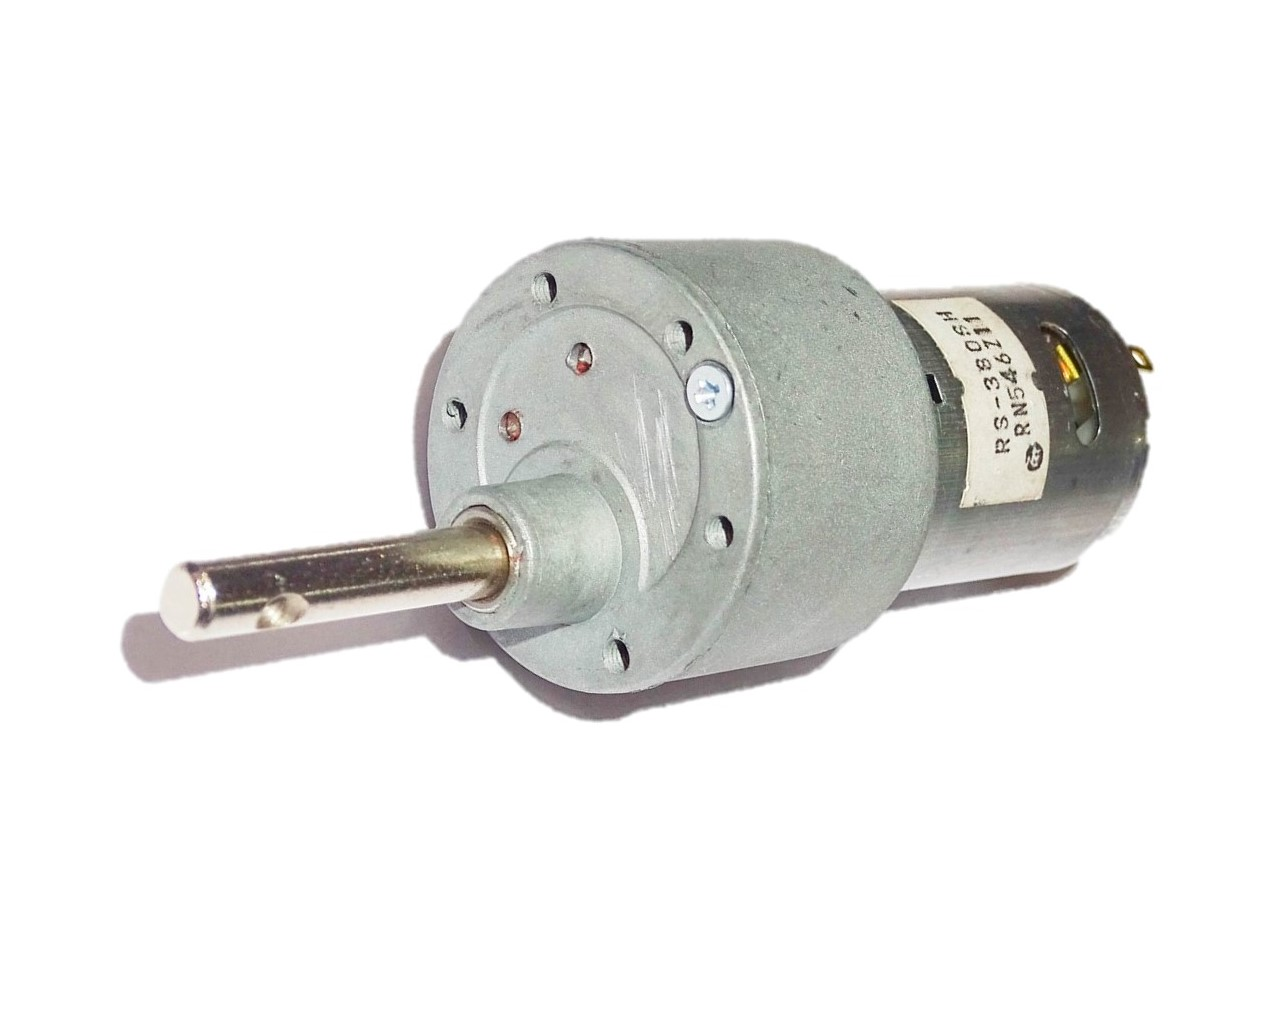
\includegraphics[width = 8cm]{project/images/johnson_motor.jpg}
    \caption{12V Johnson Geared Motor}
    \end{figure}
    
    \begin{center}{\textbf{Specifications}}\end{center}
    
    \begin{itemize}
        \item Base Motor RPM: 18000
        \item Operating Voltage: 6-18 V
        \item Rated Voltage: 12 V
        \item Rated Torque: 34.2 N-cm
        \item Stall Torque: 300 N-cm
        \item Gearbox Dimensions: 25×37 (LxW) mm
    \end{itemize}
    
    \newpage
    
    \item \textbf{Servo MG995}
    \vspace{-0.5cm}
    \paragraph{}The TowerPro MG995 High-Speed Digital Servo Motor rotates 90° in each direction making it 180° servo motor. It is a Digital Servo Motor that receives and processes PWM signal faster and better. It equips sophisticated internal circuitry that provides good torque, holding power, and faster updates in response to external forces.
    
    \begin{figure}[H]
    \centering
    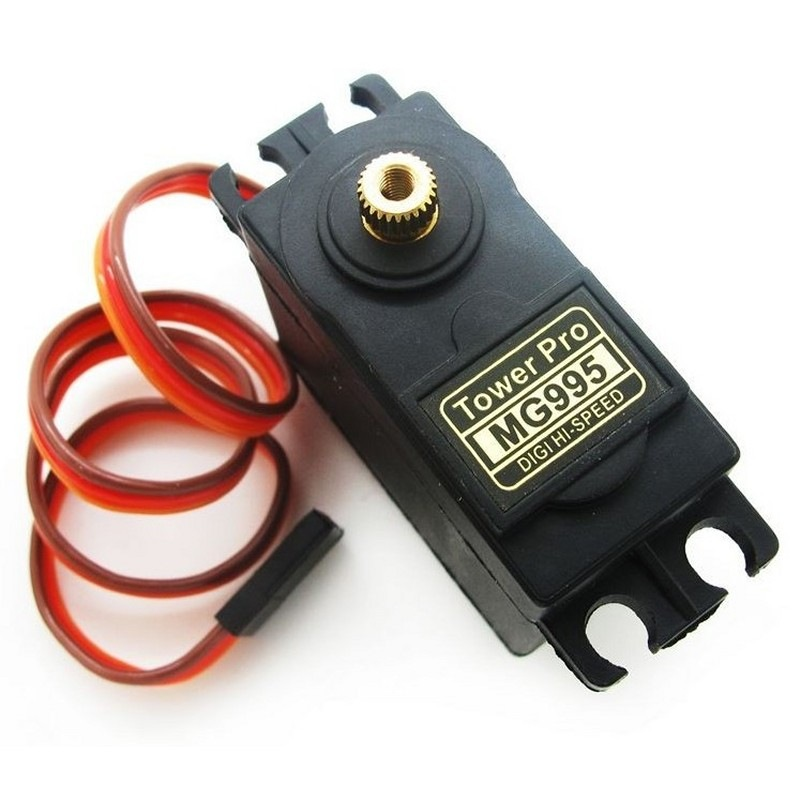
\includegraphics[width = 8cm]{project/images/mg995.jpg}
    \caption{Sevo MG995}
    \end{figure}
    
    \begin{center}{\textbf{Specifications}}\end{center}
    
    \begin{itemize}
        \item Model: MG995
        \item Weight: 55 gm
        \item Operating voltage: 4.8V~ 7.2V
        \item Servo Plug: JR
        \item Stall torque @4.8V : 10 kg-cm
        \item Stall torque @6.6V : 12 kg-cm
    \end{itemize}

\end{itemize}

\newpage

\subsection{Tri-Wheel Omni Chassis}


\begin{itemize}[wide, labelwidth=!, labelindent=0pt]
    
    \item \textbf{Omni-Wheel}
    \vspace{-0.5cm}
    \paragraph{}The 58mm Plastic Omni Wheel for Lego is the smallest Omni wheel with the loading capacity of 3kg. These wheels are compatible with Lego Motors and so with the Lego Robots. They feature rubber rollers along the circumference of the wheel which avoids slipping while moving sideways and gives minimum friction in movement.
    
    This 58mm Plastic Omni Wheel gives your Lego robot more controllable degrees of freedom as compared to conventional wheels which give only 2 degrees of freedom i.e moving forward and backward. 
    
    \begin{figure}[H]
    \centering
    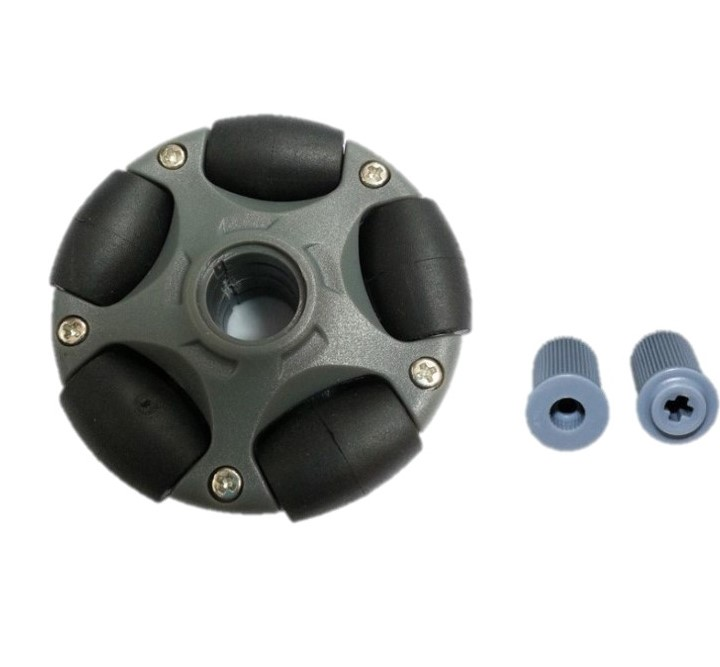
\includegraphics[width = 6cm]{project/images/omni_wheels.jpg}
    \caption{Omni Wheels}
    \end{figure}
    
    \begin{center}{\textbf{Specifications}}\end{center}
    
    \begin{itemize}
        \item Model: MG995
        \item Weight: 55 gm
        \item Operating voltage: 4.8V~ 7.2V
        \item Servo Plug: JR
        \item Stall torque @4.8V : 10 kg-cm
        \item Stall torque @6.6V : 12 kg-cm
    \end{itemize}
    
    \newpage
    
    \item \textbf{Chassis}
    \vspace{-0.5cm}
    \paragraph{} The chassis has three Omni-Wheels positioned $120^{\circ}$ each. The Omni Wheels provide easy 360° movement; with rotational and sideways maneuverability.
    
    So, what makes this wheels move in all direction? those are the small rollers along the wheel circumference. These Rollers are placed in such a way that the rotational axis of this rollers is perpendicular to the rotational axis of the main wheel. So, the Omni wheels can rotate in a forward and a backward direction like ordinary wheels and also rotate freely around itself i.e 360° rotation because of such two rotational axes within one wheel.

    \begin{figure}[H]
    \centering
    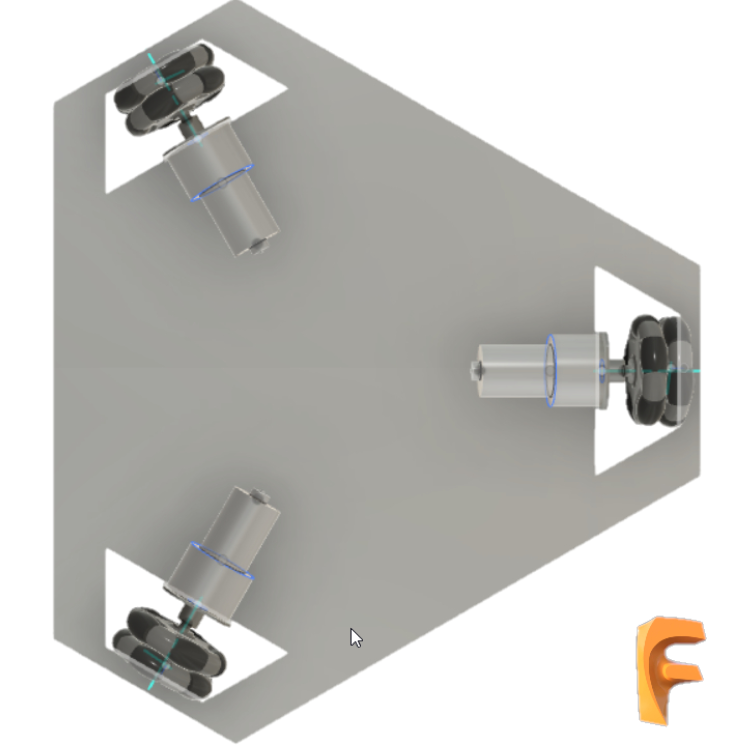
\includegraphics[width = 10cm]{project/images/chassis_3d_model.png}
    \caption{Chassis}
    \end{figure}

\end{itemize}